%======================== CHAP 4 =================

\chapter{Testing and Conclusion}
This chapter shows the results from testing the NFC evaluation module \cite{NFC_Module} in addition to a small conclusion with future improvements to the produced PCB.


\section{Testing TI datalogger}
The evaluation kit from Texas Instruments was used to test the NFC transponder chip capabilities in the following areas:

\begin{enumerate}
\item Operating modes.
\item Memory
\item Data transfer
\end{enumerate} 

\begin{figure}[h]
\begin{center}
\center
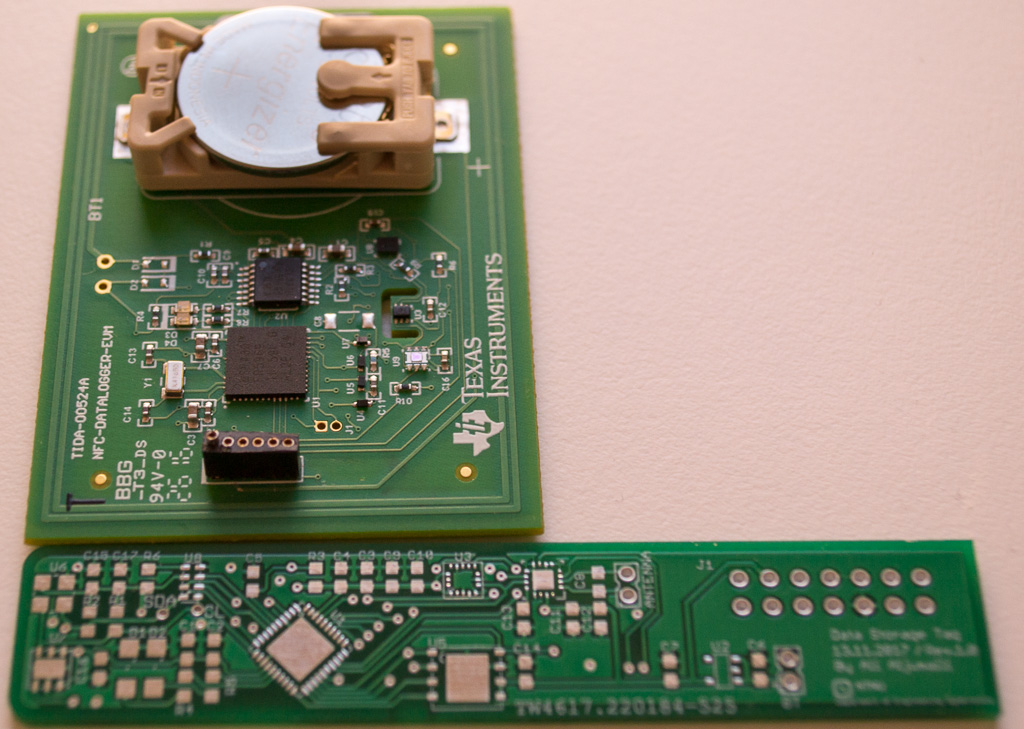
\includegraphics[scale=0.5]{Illustrations/test_prototype.jpg}  
\caption{Evaluation kit and prototype}
\label{prototype}
\end{center}
\end{figure}
\subsection{Operating mode}
The evaluation kit demonstrated successful behaviour when both reading and writing to the chip. 
The NFC Transponder chip showed that it supports ISO1443B, being able to both read and write to it using an android application and an Nexus  5X NFC enabled smartphone. 
\subsection{Memory}
The 64 KB onboard FRAM memory was capable of storing 1853 samples of time and temperature. It was tested by placing the EVM inside of a refrigerator and letting it log overnight in the cold. The memory was successfully full and all data was retrieved in the morning. Figure \ref{write_nfc} shows the application used to read and write to the chip. 


\subsection{Data transfer}
It took around 12 seconds to read the whole 64KB memory. Giving a read rate of around 5.3 KBps. This is consistent with typical data throughput of 3.2 - 5.8 KBps mentioned in the datasheet. 

Reading speed was also reasonable. The chip responded within 1-3 seconds to the written commands.
\begin{figure}[h]
\begin{center}
\center
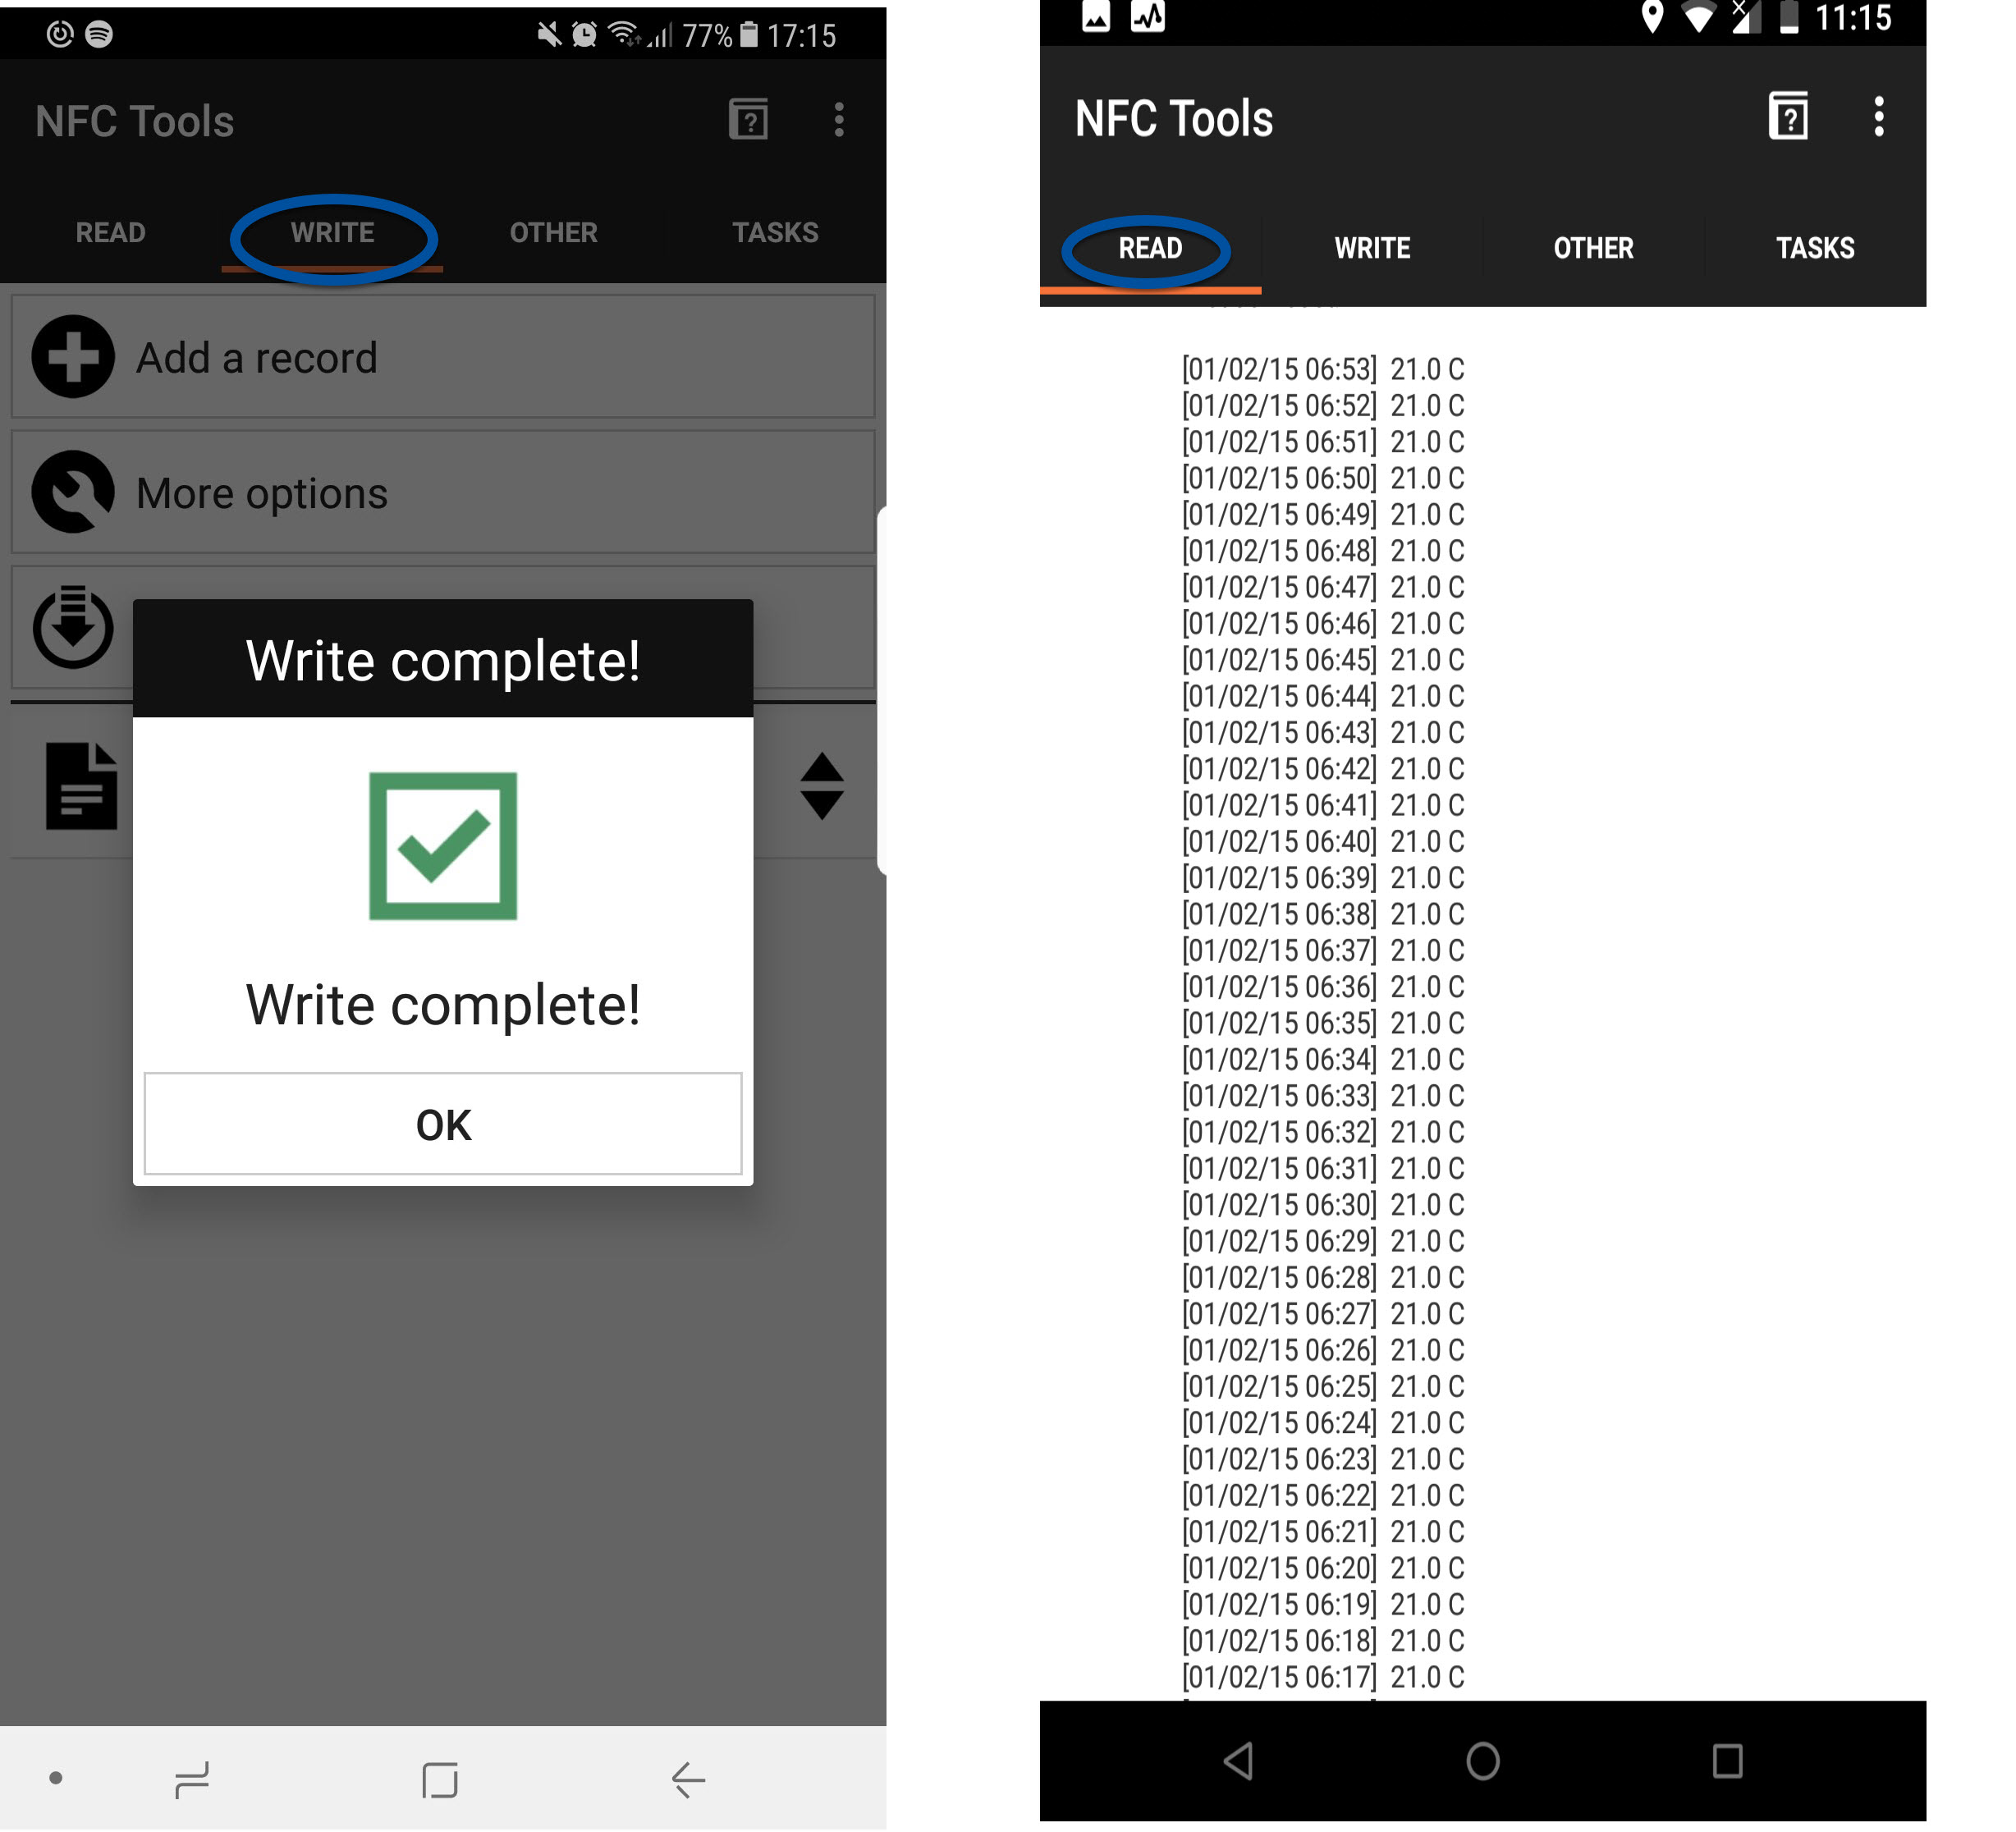
\includegraphics[scale=0.2]{Illustrations/test_data.jpg}  
\caption{Writing to the NFC Transponder using NFC tools}
\label{write_nfc}
\end{center}
\end{figure}


\section{Testing the PCB}
The PCB was tested virtually by using eagle's DRC (design rules check) to detect any air wires, crossing clearances or other showstopper mistakes. These DRC were set to match the manufacturer’s capabilities and are included in the delivered board file. An online simulator from 4pcb.com was also used to check for any showstoppers.

Testing the PCB physically was done using a multimeter, checking the copper paths for any short circuits. Multiple test points were added when designing the board to make it easy to test VCC, $I^2C$ and ground lines.  A zoom camera was also used for virtual inspection of the board.

\section{Conclusion}
After testing the NFC development kit it is shown that the RF430 NFC transponder was a good choice with reliable behaviour and low energy consumption, it was easily integrated to the $I^2C$ bus on the prototype. The PCB board was challenging because the size of the PCB, it would have been easier to use a 4 layers board with dedicated VCC and ground planes. The copper fill on the board were lacking on the edges, this should be improved in future revisions of the board. 

This project provided a good introduction to PCB design as well a good purpose for NFC technology. 
That can act as a debugging and configuration interface inside of a small devices that are sealed from the outside world, like an underwater data storage tag (DST).
